\section{Auswertung}
\label{sec:Auswertung}

\begin{figure}
  \centering
  
  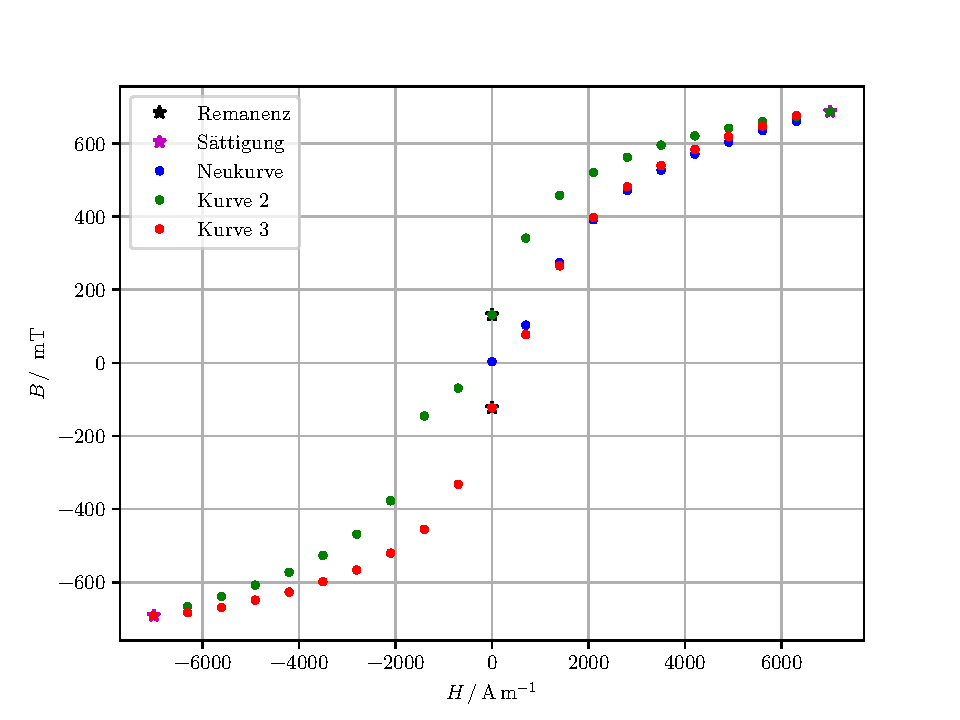
\includegraphics{hysterese.pdf}
  \caption{Messwerte der Hysteresekurve.}
  \label{fig:Hysterese}
\end{figure}



\begin{figure}
  \centering
  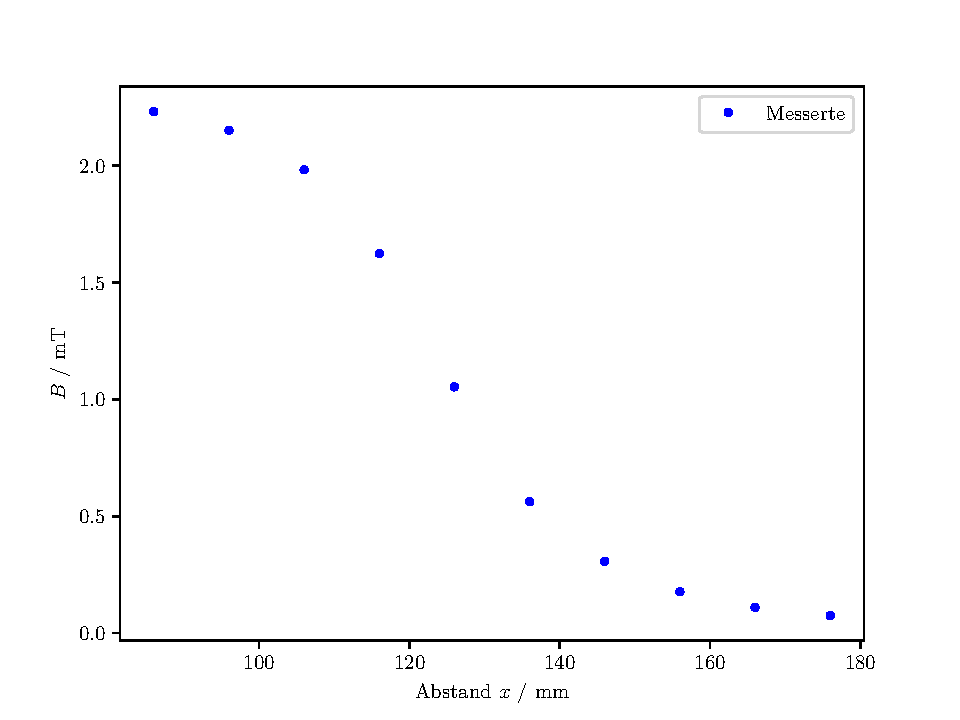
\includegraphics{langeSpule.pdf}
  \caption{Messwerte der langen Spule.}
  \label{fig:Spule}
\end{figure}



\begin{figure}
  \centering
  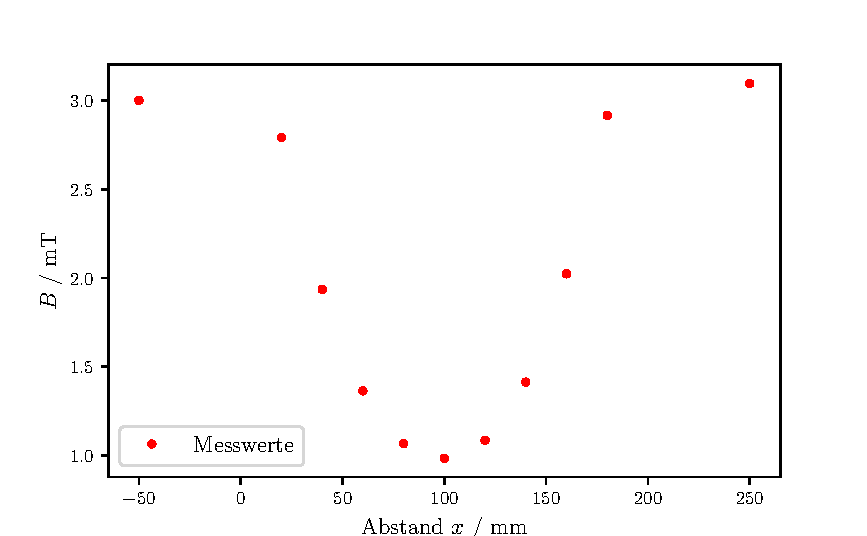
\includegraphics{Spulenpaar1.pdf}
  \caption{Messwerte des ersten Spulenpaares.}
  \label{fig:Spulenpaar1}
\end{figure}




\begin{figure}
  \centering
  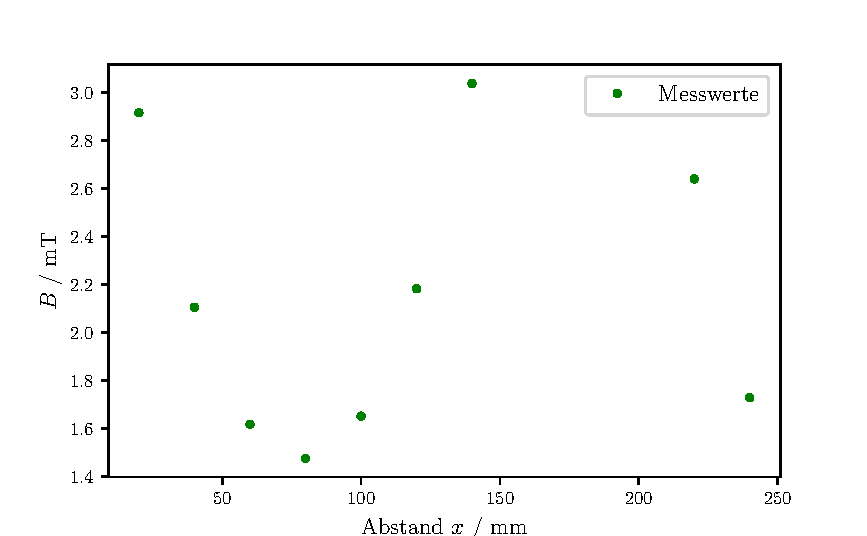
\includegraphics{Spulenpaar2.pdf}
  \caption{Messwerte des zweiten Spulenpaares.}
  \label{fig:Spulenpaar2}
\end{figure}


\begin{figure}
  \centering

  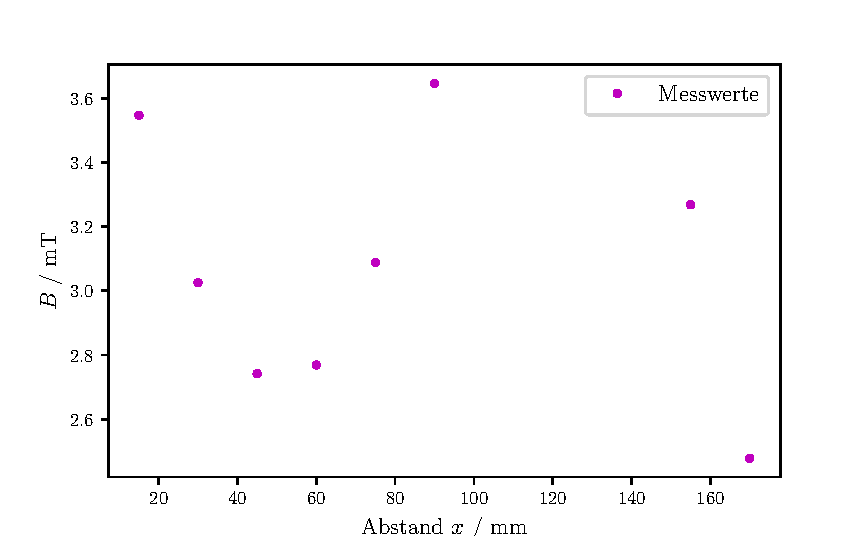
\includegraphics{Spulenpaar3.pdf}
  \caption{Messwerte des dritten Spulenpaares.}
  \label{fig:Spulenpaar3}
\end{figure}


\begin{figure}
  \centering
  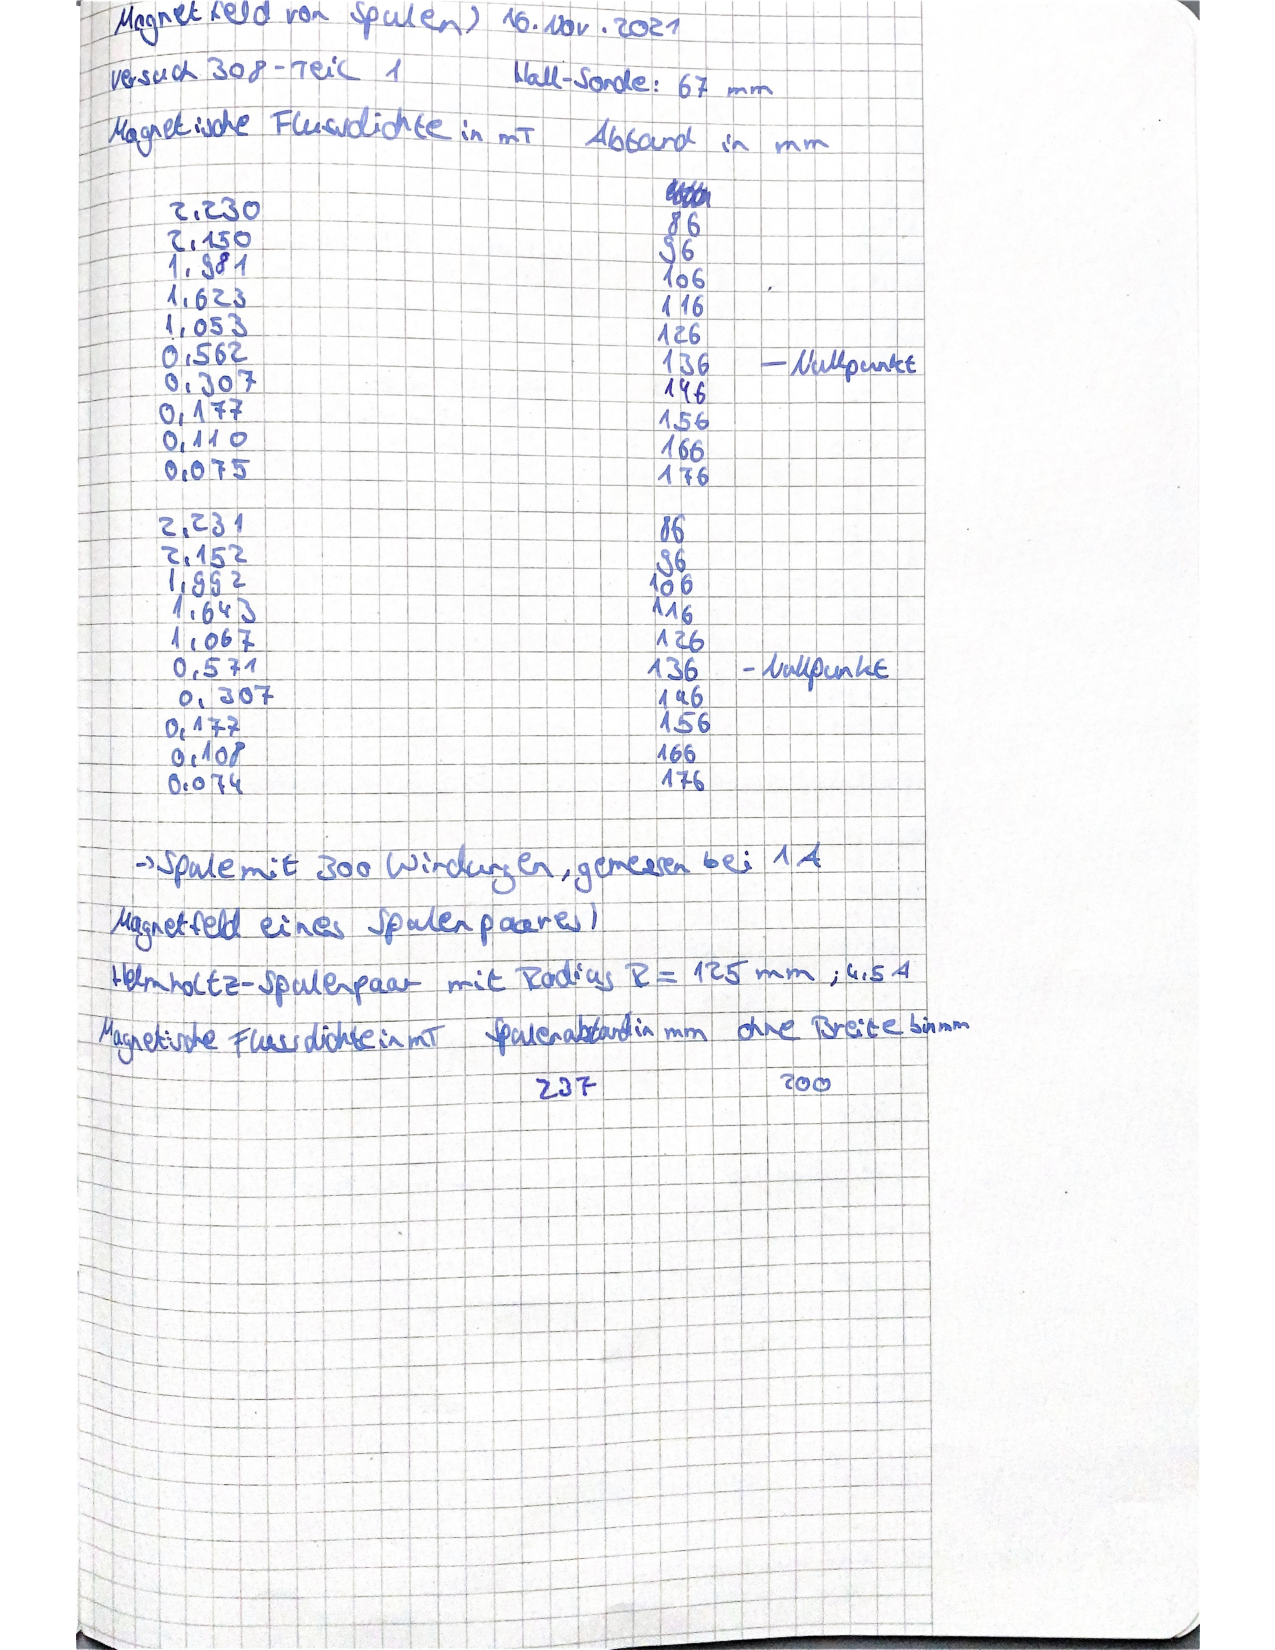
\includegraphics{daten1.pdf}
  \caption{Originale Daten aus dem Laborbuch zur langen Spule.}
  \label{fig:DatenLangeSpule}
\end{figure}

\begin{figure}
  \centering
  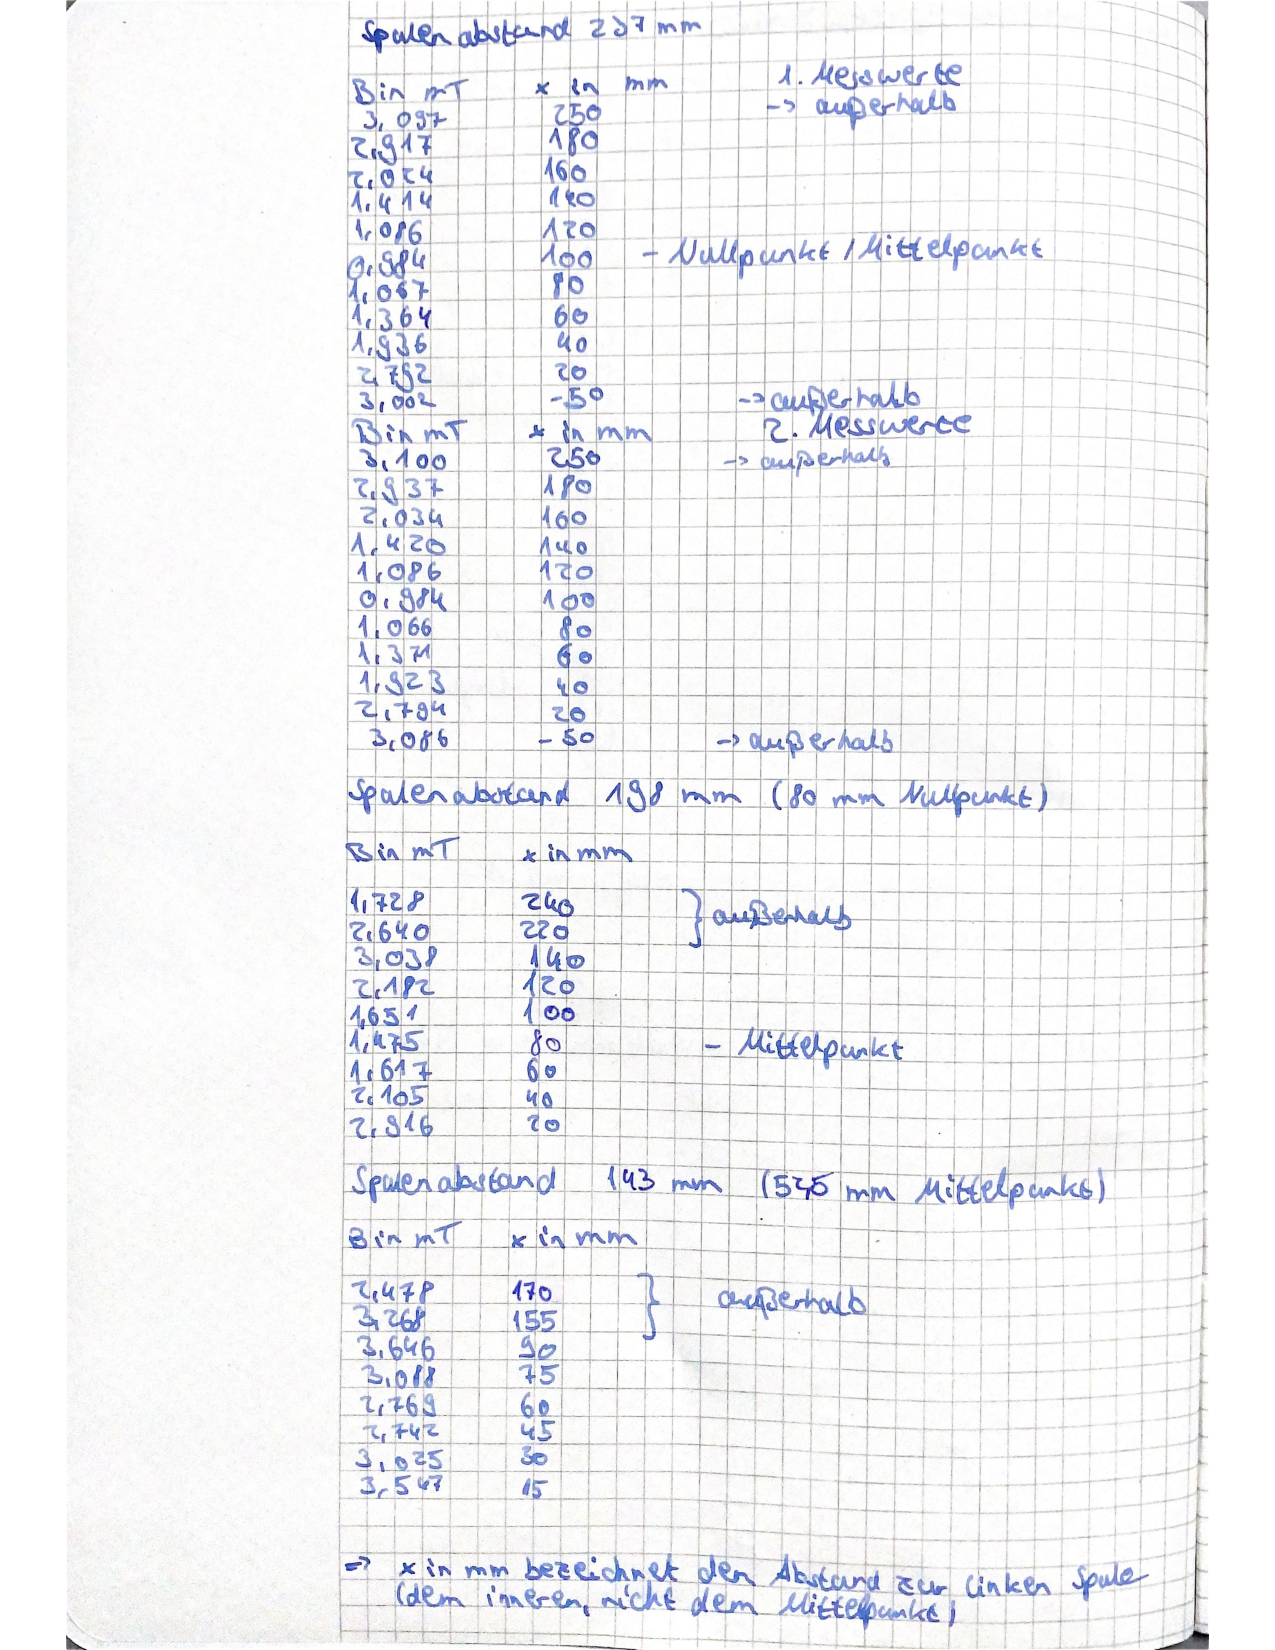
\includegraphics{daten2.pdf}
  \caption{Originale Daten aus dem Laborbuch zu den Helmholtz-Spulenpaaren.}
  \label{fig:Daten2}
\end{figure}

\begin{figure}
  \centering
  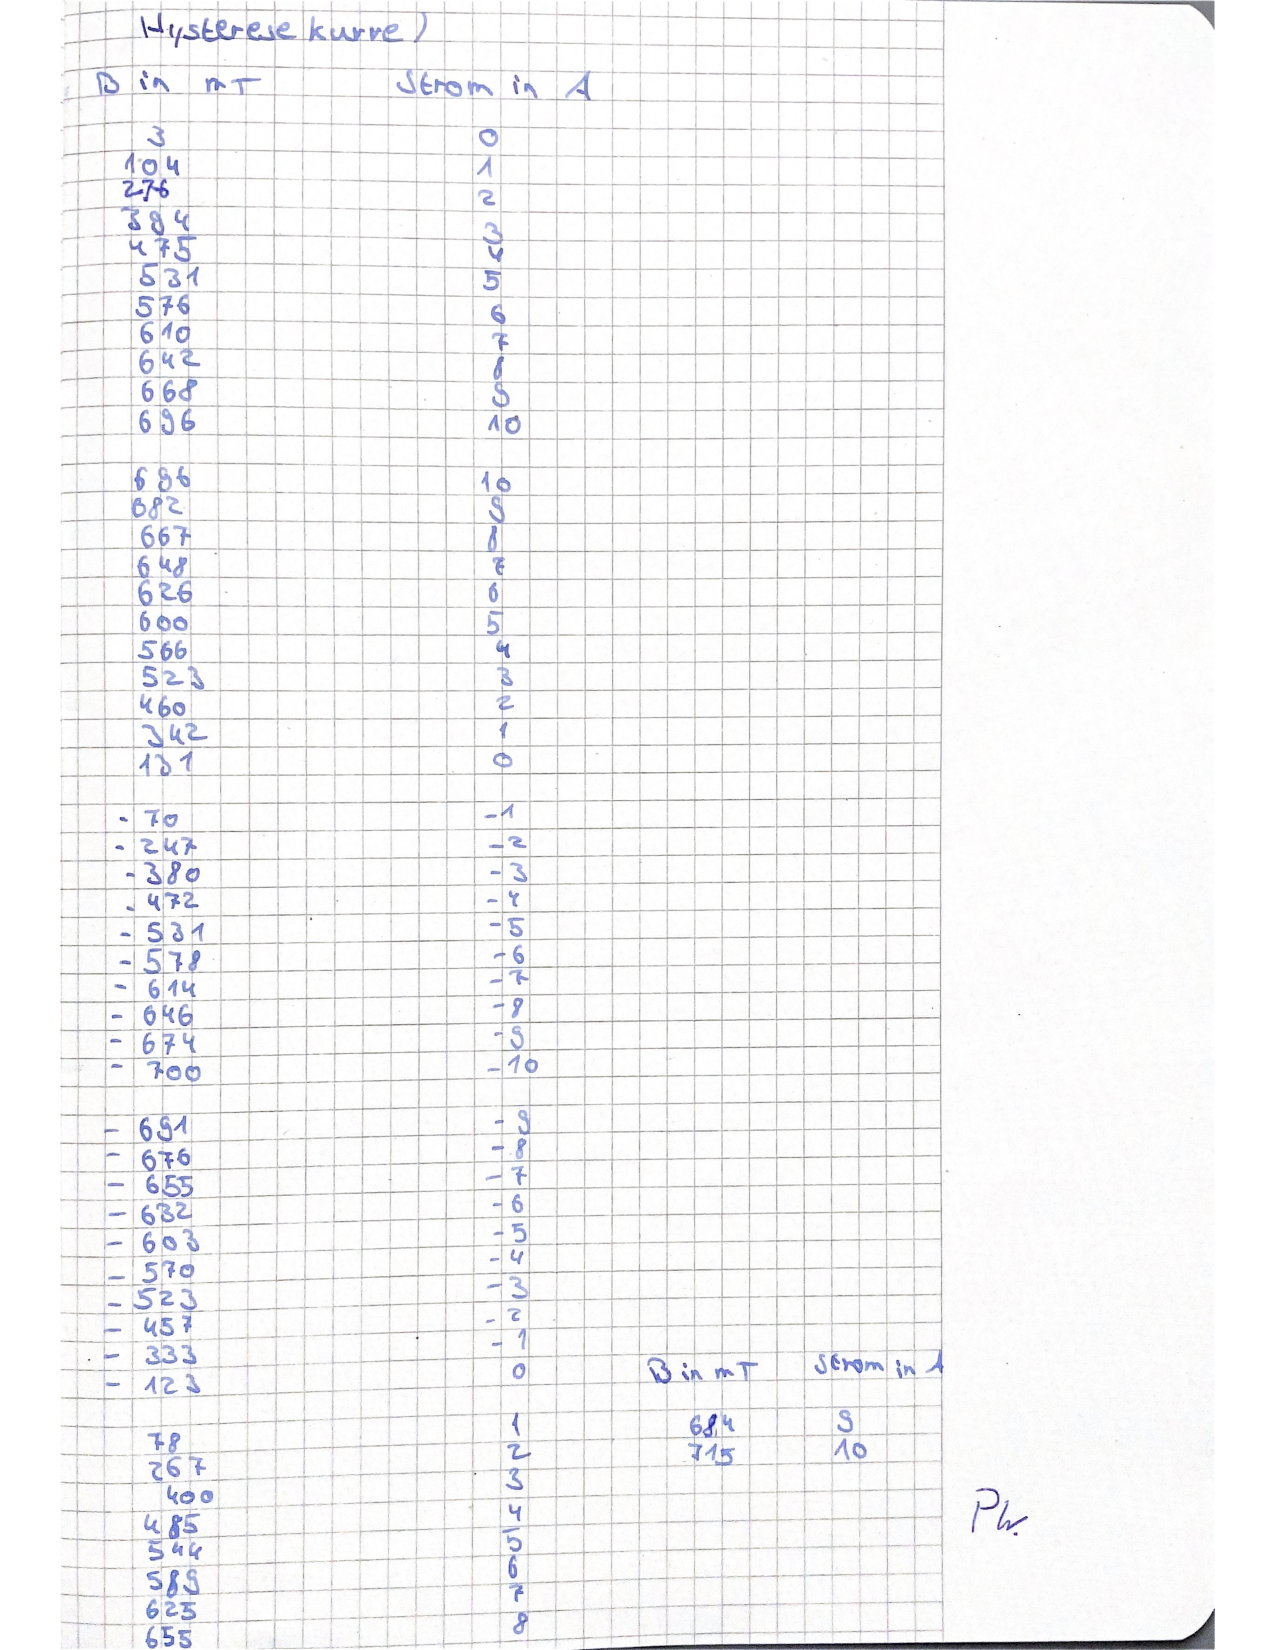
\includegraphics{daten3.pdf}
  \caption{Originale Daten aus dem Laborbuch zur hysteresekurve.}
  \label{fig:Daten3}
\end{figure}


Siehe \autoref{fig:plot}!
